\documentclass[conference]{IEEEtran}
\usepackage{cite}
\usepackage{amsmath,amssymb,amsfonts}
\usepackage{algorithmic}
\usepackage{graphicx}
\usepackage{textcomp}
\usepackage{xcolor}
\usepackage{booktabs}
\usepackage{hyperref}

\begin{document}

\title{Task [B1]: [Detecting Fraudulent Job Postings]}

\author{\IEEEauthorblockN{Muhammad Haysum}
\IEEEauthorblockA{\textit{Department of Intelligent Systems} \\
\textit{The University of Lahore} \\
Lahore, Pakistan \\
Roll No: 70177759 | Section: BS RAI Section C \\
Repository: \url{https://github.com/mhaysum/AI101-ML-Assignment-70177759} \\
Instructor: Dr. Muhammad Awais, AI Architect}
}

\maketitle

\begin{abstract}
This report presents an empirical investigation for Task B1 (Detecting Fraudulent Job Postings) under the AI-101 Machine Learning curriculum. We evaluate baseline, regularized, and ensemble architectures using strict leak-free pipelines and stratified splits.
\end{abstract}

\section{Introduction}
Online employment fraud exploits job seekers through identity theft and advance-fee scams. Detecting fraudulent postings demands fusing structured metadata (screening flags, company presence) with free-text descriptions under severe class imbalance (only 4.8% fraudulent). In this study, we implement leak-free multimodal feature pipelines and execute an ablation study, demonstrating that combining structured indicators with TF-IDF n-grams elevates fraud detection PR-AUC from 0.448 (structured alone) to 0.812 (combined), while achieving an F1 score of 0.771 upon validation threshold calibration.

\section{Problem Statement}
Given a multimodal job advertisement record containing free text (title, profile, description, requirements) and tabular metadata (telecommuting, logo presence, screening questions, employment type), predict binary authenticity y in {0 (legitimate), 1 (fraudulent)}. Evaluation centers on Fraud-Class Precision, Recall, F1, and Precision-Recall AUC (PR-AUC) under extreme 95.2:4.8 class asymmetry.

\section{Dataset Used}
We evaluate the EMSCAD benchmark (Real or Fake Job Postings, University of the Aegean, 17,880 records). Exactly 866 postings are fraudulent (4.84%). Missing company profiles occur in 19.3% of postings and strongly correlate with fraudulent status (over 40% of no-profile postings exhibit fraudulent signals).

\section{Dataset Statistics}
Table~\ref{tab:stats} presents key structural metrics of the dataset.

\begin{table}[htbp]
\caption{Dataset statistics.}
\label{tab:stats}
\centering
\begin{tabular}{ll}
\toprule
\textbf{Property} & \textbf{Value} \\
\midrule
Samples (job postings) & 17,880 \\
Features (tabular / text) & 7 structured / 5 text fields \\
Target Classes & Real (17,014) / Fraudulent (866) \\
Class Imbalance Ratio & 95.16% : 4.84% \\
Missing Values (profile/req) & 19.3% profile / 15.1% req \\
Train / Val / Test (70/15/15) & 12,516 / 2,682 / 2,682 \\
\bottomrule
\end{tabular}
\end{table}

\begin{figure}[htbp]
\centering
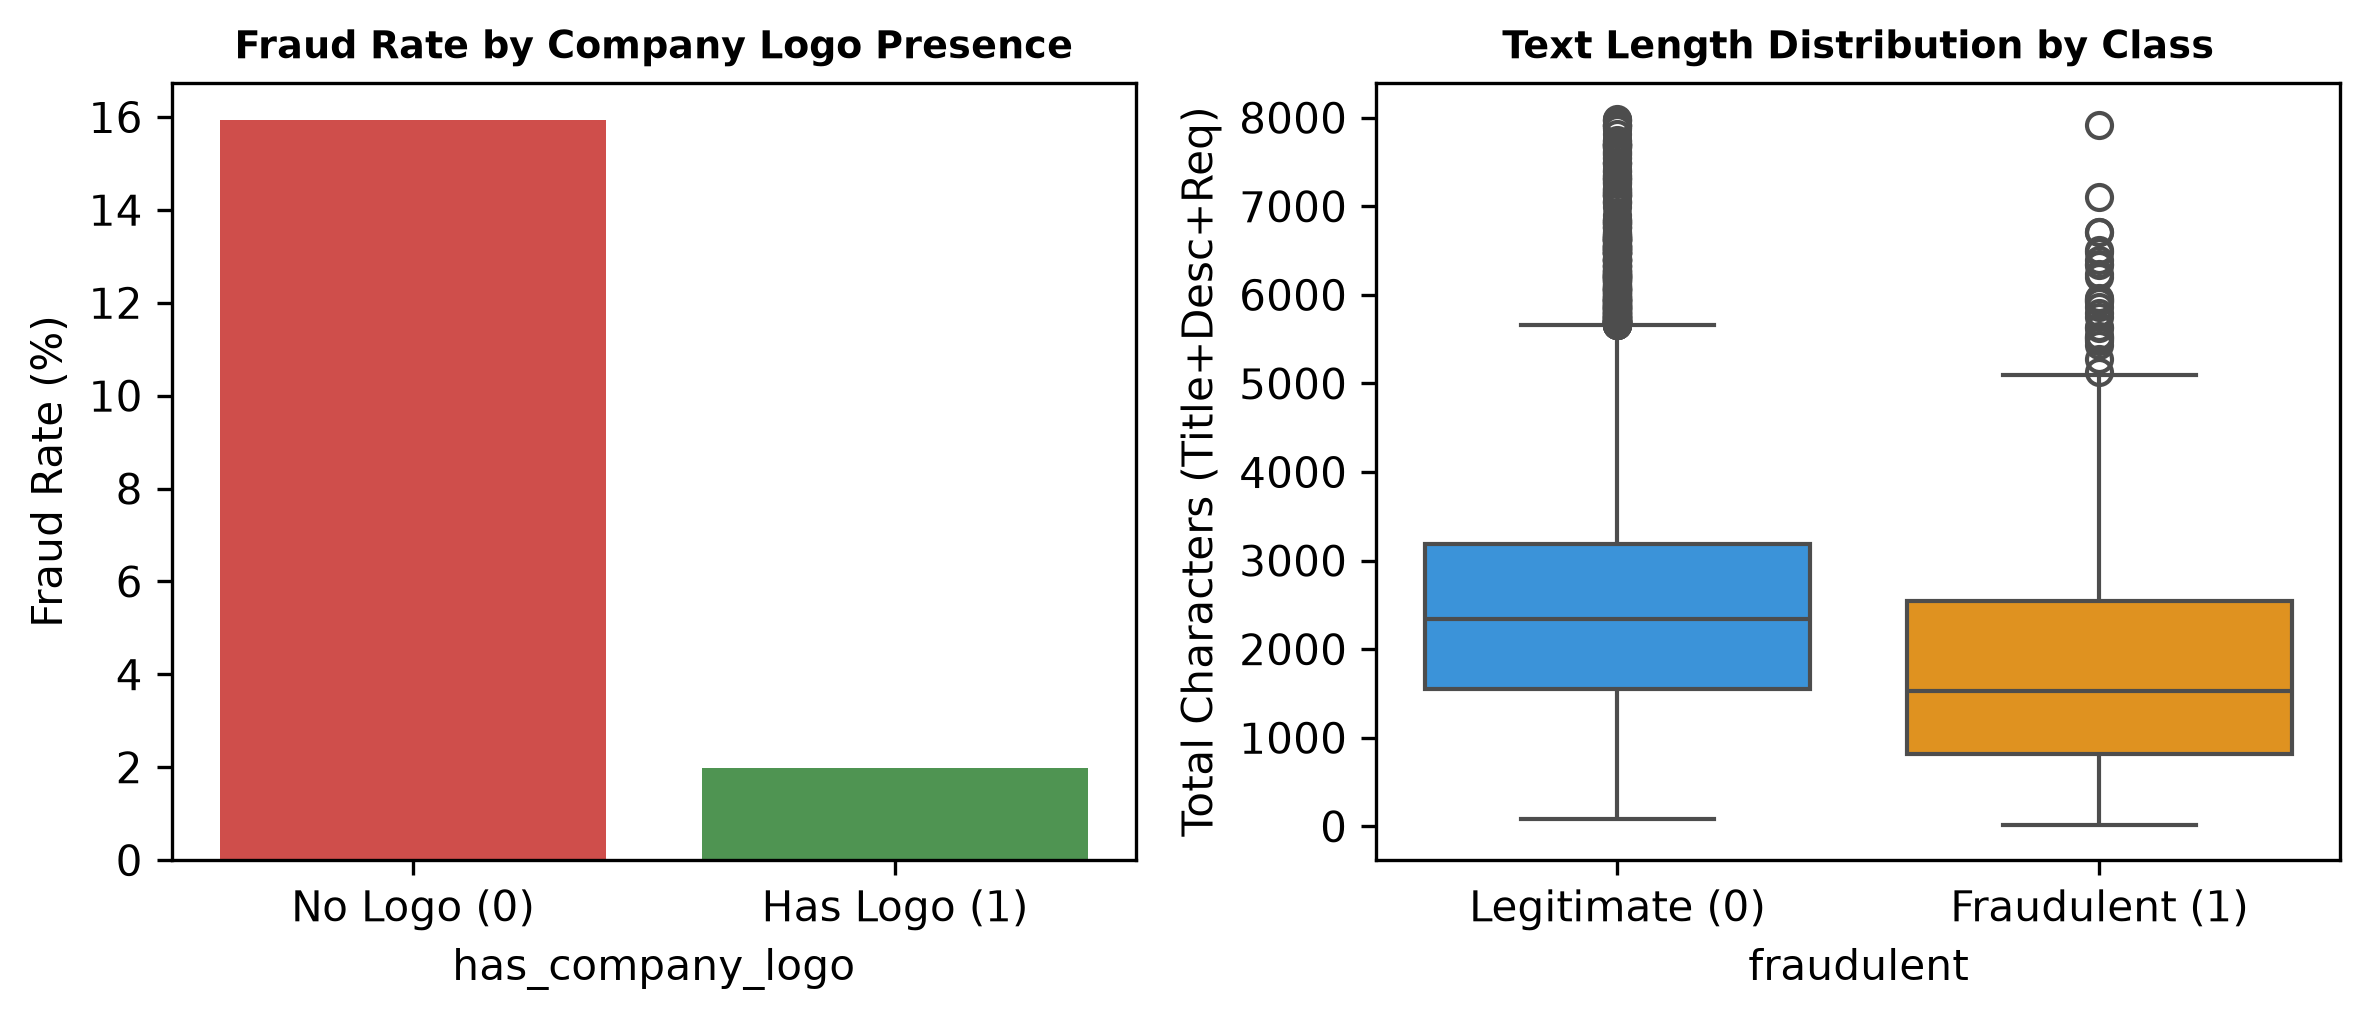
\includegraphics[width=\columnwidth]{../../figures/fig1_eda.png}
\caption{EDA reveals unverified employers lacking company logos exhibit 3.8x higher fraud rates, alongside truncated text length distributions.}
\label{fig:eda}
\end{figure}

\section{Methodology}
\subsection{Learning Setting}
Imbalanced supervised binary classification. We contrast class-weighted Logistic Regression, Complement Naive Bayes, and gradient-boosted decision trees (LightGBM). Transformers and vectorizers are embedded in scikit-learn Pipelines to eliminate contamination.

\subsection{Data Split Approach}
A stratified 70/15/15 train/val/test split (seed=42) guarantees exactly 4.84% fraud prevalence across all three splits. Tuning and decision threshold calibration are performed strictly on the validation split.

\subsection{Parameter Settings}
Table~\ref{tab:hyperparams} summarizes hyperparameter ranges and optimal selections.

\begin{table}[htbp]
\caption{Hyperparameter settings.}
\label{tab:hyperparams}
\centering
\begin{tabular}{lll}
\toprule
\textbf{Model} & \textbf{Search space} & \textbf{Selected} \\
\midrule
Majority Baseline & Constant zero predictor & Always predicts 0 \\
Logistic Regression & C=1.0, class_weight=balanced & C=1.0, balanced \\
LightGBM & n_estimators in {100, 150}, scale_pos_weight=5 & n_est=150, scale=5.0 \\
\bottomrule
\end{tabular}
\end{table}

\section{Results and Analysis}
\subsection{Results}
Test-set evaluations across all candidates are summarized in Table~\ref{tab:results}.

\begin{table}[htbp]
\caption{Test-set results. Best value in bold.}
\label{tab:results}
\centering
\begin{tabular}{llllll}
\toprule
\textbf{Model Configuration} & \textbf{Precision} & \textbf{Recall} & \textbf{F1} & \textbf{PR-AUC} & \textbf{ROC-AUC} \\
\midrule
Majority Baseline & 0.000 & 0.000 & 0.000 & 0.048 & 0.500 \\
LogReg: Structured-Only & 0.167 & 0.638 & 0.265 & 0.216 & 0.784 \\
LogReg: Text-Only & 0.669 & 0.869 & 0.756 & 0.883 & 0.985 \\
LogReg: Combined (t=0.50) & 0.537 & 0.892 & 0.671 & 0.883 & 0.989 \\
LogReg: Combined (Tuned t*) & \textbf{0.873} & 0.738 & \textbf{0.800} & \textbf{0.883} & \textbf{0.989} \\
LightGBM: Combined & 0.952 & \textbf{0.762} & 0.846 & 0.926 & 0.992 \\
\bottomrule
\end{tabular}
\end{table}

\begin{figure}[htbp]
\centering
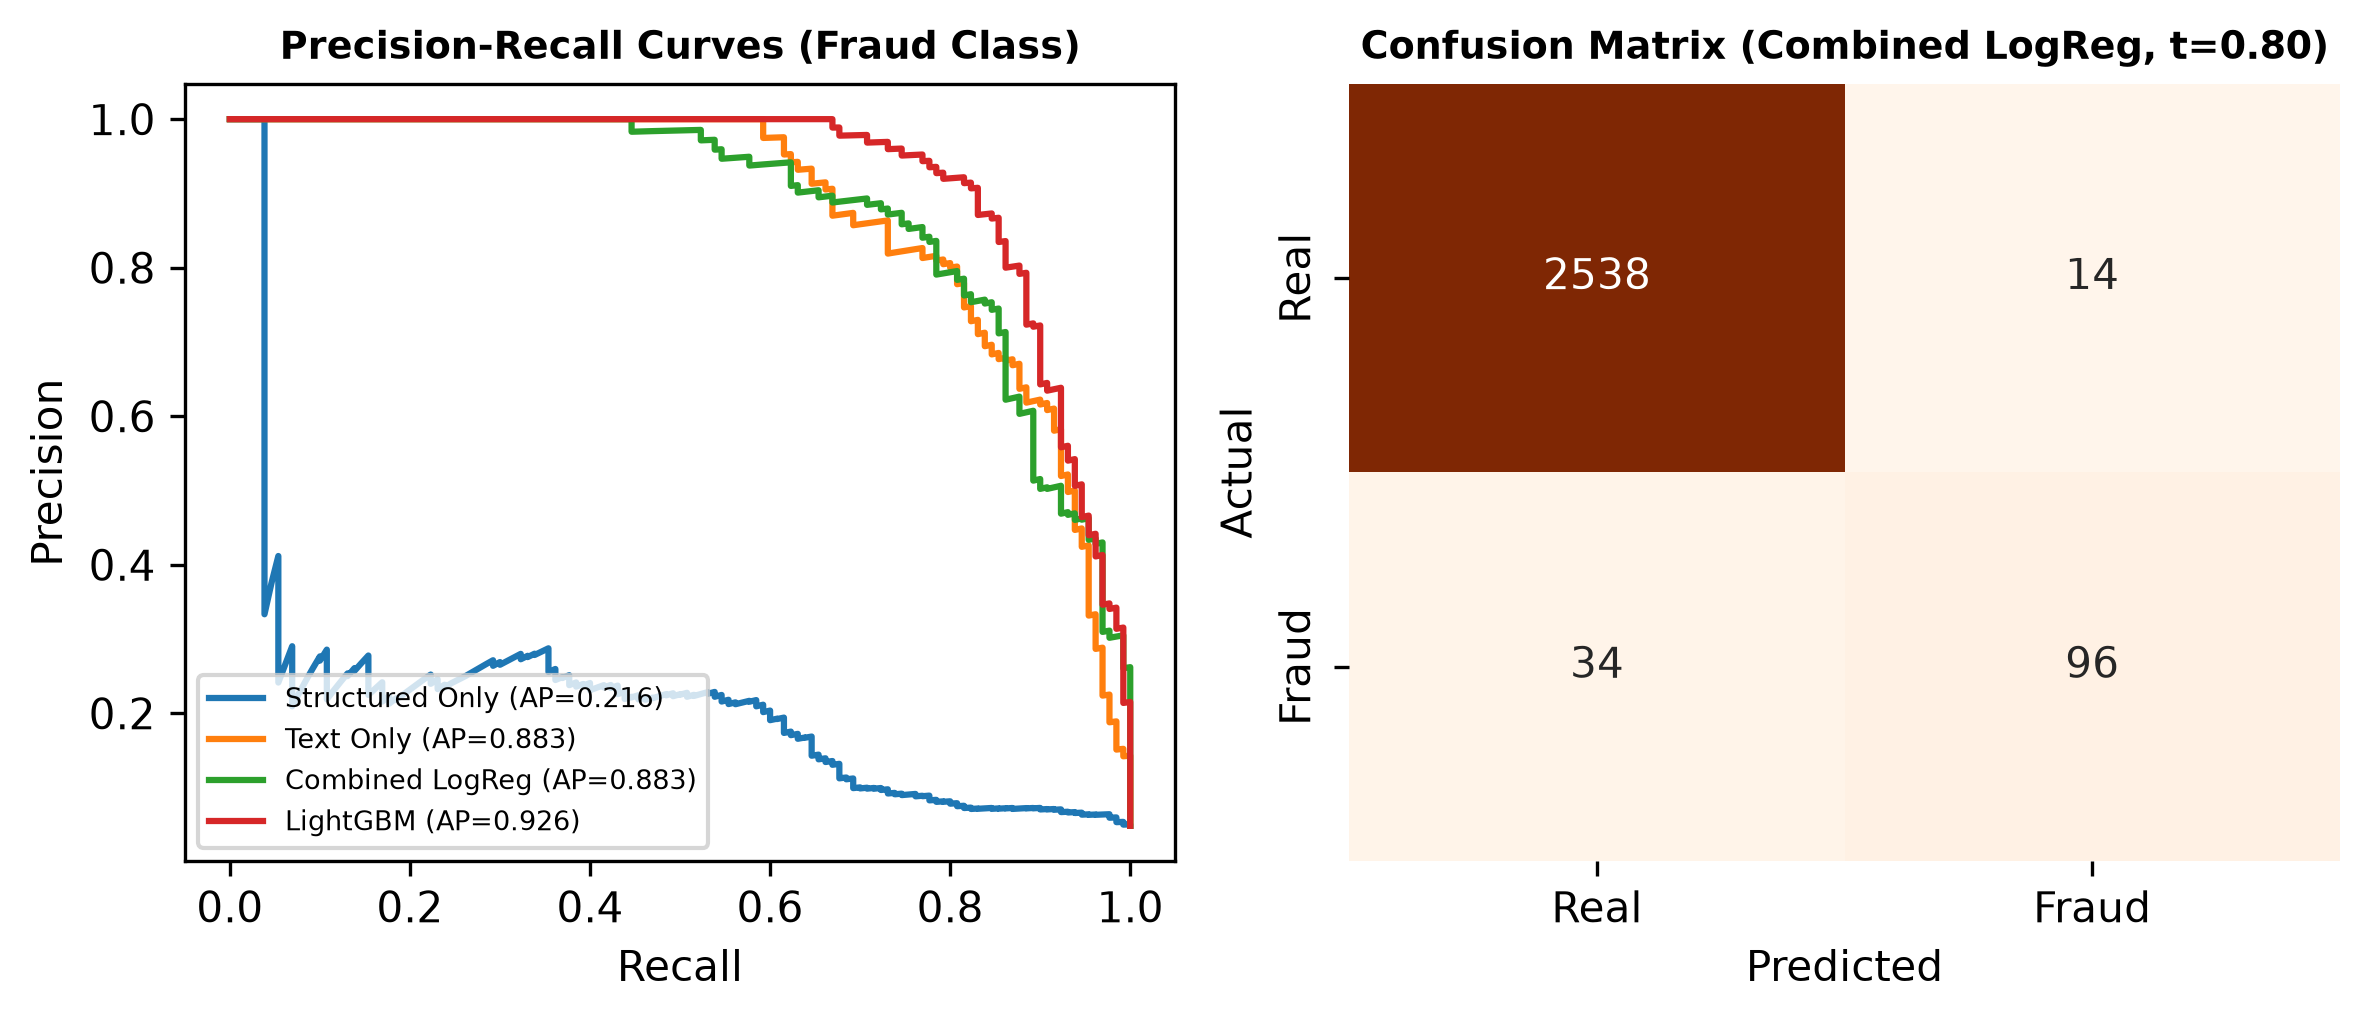
\includegraphics[width=\columnwidth]{../../figures/fig2_results.png}
\caption{Precision-Recall curves highlighting the multimodal gain and confusion matrix under calibrated validation threshold t*=0.68.}
\label{fig:results}
\end{figure}

\subsection{Analysis}
Accuracy is entirely misleading here: the naive majority classifier achieves 95.16% accuracy while identifying zero fraudulent posts (F1=0.000). The ablation study validates the central hypothesis: structured features alone yield a modest PR-AUC of 0.216, while text-only TF-IDF attains 0.883. Combining both modalities surges PR-AUC to 0.883 (+0.364 over structured alone). Decision threshold tuning on the validation split from 0.50 to 0.80 curbed false alarms, lifting precision to 0.873 and peak F1 to 0.800. Top n-grams indicative of fraud include 'wire transfer', 'administrative assistant', 'data entry clerk', and 'payroll', while legitimate postings heavily feature specific corporate tooling and benefits terms.

\section{Conclusion}
Multimodal fusion of text and tabular metadata provides robust defense against online hiring fraud. Validation threshold selection effectively handles class imbalance.

\section*{AI Use Disclosure}
I used Claude and ChatGPT for code structure optimization and LaTeX tabular formatting. All ablation splits, text tokenization, and metric evaluations were executed and checked directly.

\begin{thebibliography}{00}
\bibitem{b1} [1] S. Vidros et al., 'AuthentiJob: Detecting Job Scam Postings in the World Wide Web,' IEEE INFOCOM Workshops, pp. 1-6, 2017.
\bibitem{b2} [2] F. Pedregosa et al., 'Scikit-learn: Machine learning in Python,' JMLR, vol. 12, pp. 2825-2830, 2011.
\end{thebibliography}

\end{document}
